\documentclass{standalone}
\usepackage{tikz}
\usetikzlibrary{patterns, positioning}
\usepackage[sfdefault]{ClearSans} %% option 'sfdefault' activates Clear Sans as the default text font
\usepackage[T1]{fontenc}

\begin{document}
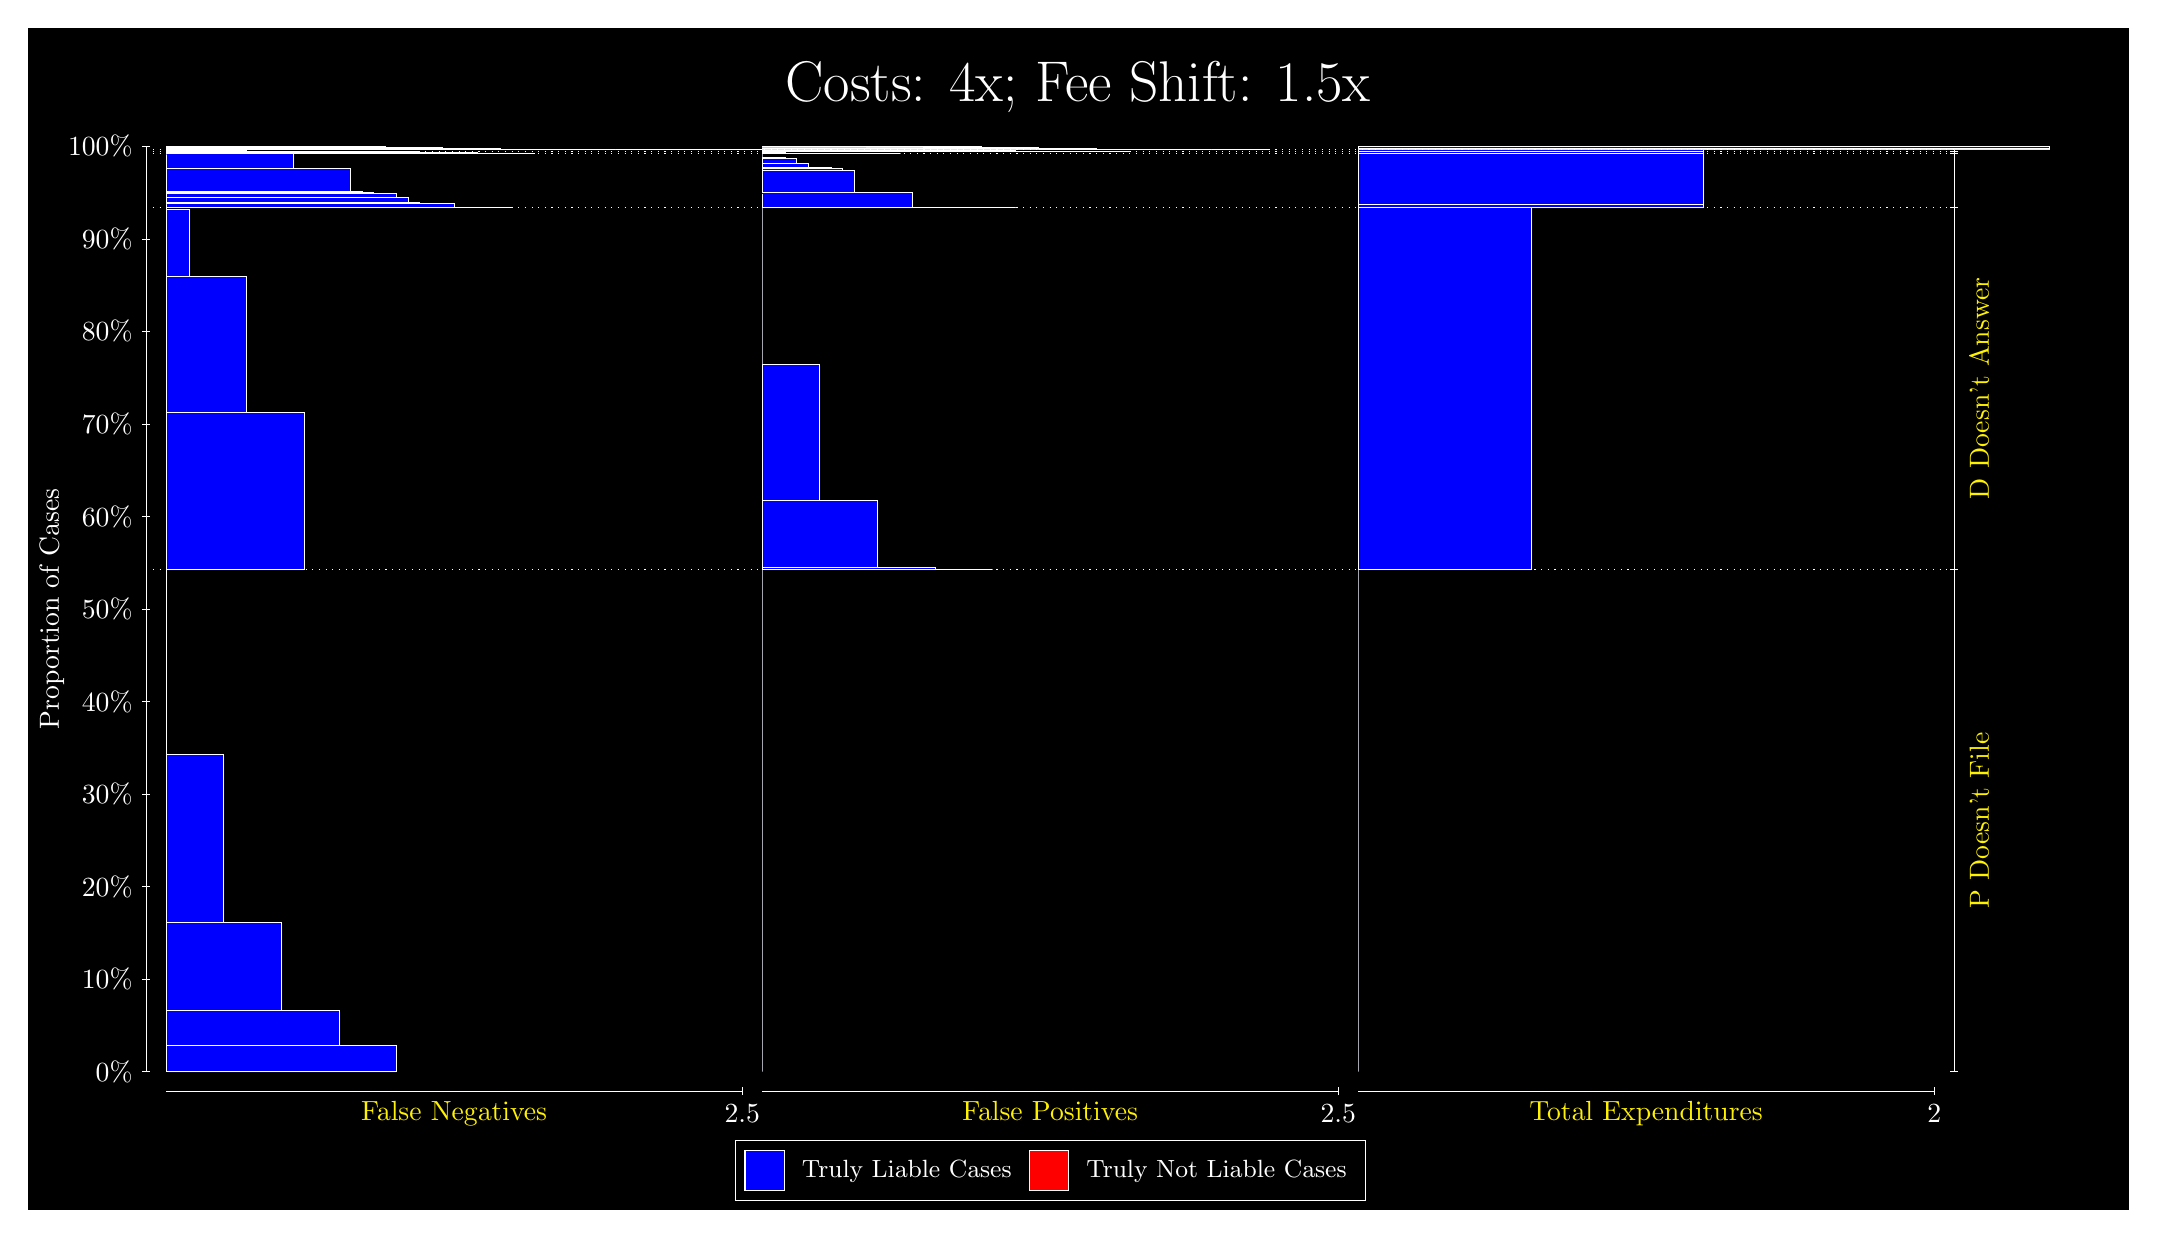
\begin{tikzpicture}
\draw[fill=black] (0,0) rectangle (26.667,15);
\draw[text=white] (0,13.5) rectangle (26.667,15) node[midway] {\huge Costs: 4x; Fee Shift: 1.5x};
\draw[white, very thin] (1.5,1.75) -- (1.5,13.5);
\node[rotate=90, text=white, anchor=center] at (0.3, 7.625) {Proportion of Cases};
\draw[white, very thin] (1.45,1.75) -- (1.55,1.75);
\node[text=white, anchor=east] at (1.45, 1.75) {0\%};
\draw[white, very thin] (1.45,2.925) -- (1.55,2.925);
\node[text=white, anchor=east] at (1.45, 2.925) {10\%};
\draw[white, very thin] (1.45,4.1) -- (1.55,4.1);
\node[text=white, anchor=east] at (1.45, 4.1) {20\%};
\draw[white, very thin] (1.45,5.275) -- (1.55,5.275);
\node[text=white, anchor=east] at (1.45, 5.275) {30\%};
\draw[white, very thin] (1.45,6.45) -- (1.55,6.45);
\node[text=white, anchor=east] at (1.45, 6.45) {40\%};
\draw[white, very thin] (1.45,7.625) -- (1.55,7.625);
\node[text=white, anchor=east] at (1.45, 7.625) {50\%};
\draw[white, very thin] (1.45,8.8) -- (1.55,8.8);
\node[text=white, anchor=east] at (1.45, 8.8) {60\%};
\draw[white, very thin] (1.45,9.975) -- (1.55,9.975);
\node[text=white, anchor=east] at (1.45, 9.975) {70\%};
\draw[white, very thin] (1.45,11.15) -- (1.55,11.15);
\node[text=white, anchor=east] at (1.45, 11.15) {80\%};
\draw[white, very thin] (1.45,12.325) -- (1.55,12.325);
\node[text=white, anchor=east] at (1.45, 12.325) {90\%};
\draw[white, very thin] (1.45,13.5) -- (1.55,13.5);
\node[text=white, anchor=east] at (1.45, 13.5) {100\%};

\draw[white, very thin] (24.457,1.75) -- (24.457,13.5);
\draw[white, very thin] (24.407,1.75) -- (24.507,1.75);
\node[anchor=west] at (24.407, 1.75) {};
\draw[white, very thin] (24.407,8.1283) -- (24.507,8.1283);
\node[anchor=west] at (24.407, 8.1283) {};
\draw[white, very thin] (24.407,12.725) -- (24.507,12.725);
\node[anchor=west] at (24.407, 12.725) {};
\draw[white, very thin] (24.407,13.409) -- (24.507,13.409);
\node[anchor=west] at (24.407, 13.409) {};
\draw[white, very thin] (24.407,13.438) -- (24.507,13.438);
\node[anchor=west] at (24.407, 13.438) {};
\draw[white, very thin] (24.407,13.463) -- (24.507,13.463);
\node[anchor=west] at (24.407, 13.463) {};
\draw[white, very thin] (24.407,13.5) -- (24.507,13.5);
\node[anchor=west] at (24.407, 13.5) {};

\draw[white, very thin, fill=blue] (1.75,1.75) rectangle (4.6775,2.0868);
\draw[white, very thin, fill=blue] (1.75,2.0868) rectangle (3.9457,2.531);
\draw[white, very thin, fill=blue] (1.75,2.531) rectangle (3.2138,3.6447);
\draw[white, very thin, fill=blue] (1.75,3.6447) rectangle (2.4819,5.7805);
\draw[white, very thin, fill=red] (1.75,5.7805) rectangle (1.75,5.7805);
\draw[white, very thin, fill=blue] (1.75,5.7805) rectangle (1.75,8.1283);
\draw[white, very thin, fill=blue] (1.75,8.1283) rectangle (3.5065,10.123);
\draw[white, very thin, fill=blue] (1.75,10.123) rectangle (2.7746,11.853);
\draw[white, very thin, fill=blue] (1.75,11.853) rectangle (2.0428,12.697);
\draw[white, very thin, fill=red] (1.75,12.697) rectangle (1.75,12.697);
\draw[white, very thin, fill=blue] (1.75,12.697) rectangle (1.75,12.725);
\draw[white, very thin, fill=blue] (1.75,12.725) rectangle (6.1413,12.726);
\draw[white, very thin, fill=blue] (1.75,12.726) rectangle (5.8486,12.726);
\draw[white, very thin, fill=blue] (1.75,12.726) rectangle (5.5558,12.728);
\draw[white, very thin, fill=blue] (1.75,12.728) rectangle (5.4094,12.771);
\draw[white, very thin, fill=blue] (1.75,12.771) rectangle (5.2631,12.771);
\draw[white, very thin, fill=blue] (1.75,12.771) rectangle (5.1167,12.776);
\draw[white, very thin, fill=blue] (1.75,12.776) rectangle (4.9703,12.79);
\draw[white, very thin, fill=blue] (1.75,12.79) rectangle (4.8239,12.849);
\draw[white, very thin, fill=blue] (1.75,12.849) rectangle (4.6775,12.903);
\draw[white, very thin, fill=blue] (1.75,12.903) rectangle (4.5312,12.905);
\draw[white, very thin, fill=blue] (1.75,12.905) rectangle (4.3848,12.911);
\draw[white, very thin, fill=blue] (1.75,12.911) rectangle (4.2384,12.933);
\draw[white, very thin, fill=blue] (1.75,12.933) rectangle (4.092,13.22);
\draw[white, very thin, fill=blue] (1.75,13.22) rectangle (3.9457,13.22);
\draw[white, very thin, fill=blue] (1.75,13.22) rectangle (3.7993,13.222);
\draw[white, very thin, fill=blue] (1.75,13.222) rectangle (3.6529,13.222);
\draw[white, very thin, fill=blue] (1.75,13.222) rectangle (3.5065,13.223);
\draw[white, very thin, fill=blue] (1.75,13.223) rectangle (3.3602,13.407);
\draw[white, very thin, fill=blue] (1.75,13.407) rectangle (3.2138,13.407);
\draw[white, very thin, fill=blue] (1.75,13.407) rectangle (3.0674,13.407);
\draw[white, very thin, fill=blue] (1.75,13.407) rectangle (2.921,13.407);
\draw[white, very thin, fill=blue] (1.75,13.407) rectangle (2.7746,13.407);
\draw[white, very thin, fill=blue] (1.75,13.407) rectangle (2.6283,13.409);
\draw[white, very thin, fill=blue] (1.75,13.409) rectangle (2.3355,13.409);
\draw[white, very thin, fill=blue] (1.75,13.409) rectangle (2.0428,13.409);
\draw[white, very thin, fill=red] (1.75,13.409) rectangle (1.75,13.409);
\draw[white, very thin, fill=blue] (1.75,13.409) rectangle (6.4341,13.409);
\draw[white, very thin, fill=blue] (1.75,13.409) rectangle (5.7022,13.422);
\draw[white, very thin, fill=blue] (1.75,13.422) rectangle (4.9703,13.438);
\draw[white, very thin, fill=blue] (1.75,13.438) rectangle (4.2384,13.438);
\draw[white, very thin, fill=blue] (1.75,13.438) rectangle (3.5065,13.438);
\draw[white, very thin, fill=red] (1.75,13.438) rectangle (1.75,13.438);
\draw[white, very thin, fill=blue] (1.75,13.438) rectangle (3.5065,13.438);
\draw[white, very thin, fill=blue] (1.75,13.438) rectangle (2.7746,13.454);
\draw[white, very thin, fill=blue] (1.75,13.454) rectangle (2.0428,13.463);
\draw[white, very thin, fill=red] (1.75,13.463) rectangle (1.75,13.463);
\draw[white, very thin, fill=blue] (1.75,13.463) rectangle (1.75,13.463);
\draw[white, very thin, fill=blue] (1.75,13.463) rectangle (13.46,13.463);
\draw[white, very thin, fill=blue] (1.75,13.463) rectangle (12.728,13.463);
\draw[white, very thin, fill=blue] (1.75,13.463) rectangle (11.996,13.463);
\draw[white, very thin, fill=blue] (1.75,13.463) rectangle (11.265,13.467);
\draw[white, very thin, fill=blue] (1.75,13.467) rectangle (10.533,13.467);
\draw[white, very thin, fill=blue] (1.75,13.467) rectangle (9.8008,13.467);
\draw[white, very thin, fill=blue] (1.75,13.467) rectangle (9.0689,13.467);
\draw[white, very thin, fill=blue] (1.75,13.467) rectangle (7.4587,13.467);
\draw[white, very thin, fill=blue] (1.75,13.467) rectangle (6.7268,13.467);
\draw[white, very thin, fill=blue] (1.75,13.467) rectangle (5.9949,13.473);
\draw[white, very thin, fill=blue] (1.75,13.473) rectangle (5.2631,13.491);
\draw[white, very thin, fill=blue] (1.75,13.491) rectangle (4.5312,13.5);
\draw[white, very thin, fill=blue] (1.75,13.5) rectangle (3.7993,13.5);
\draw[white, very thin, fill=blue] (1.75,13.5) rectangle (3.0674,13.5);
\draw[white, very thin, fill=blue] (1.75,13.5) rectangle (2.3355,13.5);
\draw[white, very thin, fill=red] (1.75,13.5) rectangle (1.75,13.5);
\draw[white, very thin, fill=red] (9.3189,1.75) rectangle (9.3189,1.75);
\draw[white, very thin, fill=blue] (9.3189,1.75) rectangle (9.3189,8.1283);
\draw[white, very thin, fill=red] (9.3189,8.1283) rectangle (12.246,8.1283);
\draw[white, very thin, fill=blue] (9.3189,8.1283) rectangle (12.246,8.1283);
\draw[white, very thin, fill=blue] (9.3189,8.1283) rectangle (11.515,8.1569);
\draw[white, very thin, fill=blue] (9.3189,8.1569) rectangle (10.783,9.0008);
\draw[white, very thin, fill=blue] (9.3189,9.0008) rectangle (10.051,10.73);
\draw[white, very thin, fill=blue] (9.3189,10.73) rectangle (9.3189,12.725);
\draw[white, very thin, fill=red] (9.3189,12.725) rectangle (12.539,12.725);
\draw[white, very thin, fill=blue] (9.3189,12.725) rectangle (12.539,12.725);
\draw[white, very thin, fill=red] (9.3189,12.725) rectangle (12.246,12.725);
\draw[white, very thin, fill=blue] (9.3189,12.725) rectangle (12.246,12.725);
\draw[white, very thin, fill=red] (9.3189,12.725) rectangle (11.954,12.725);
\draw[white, very thin, fill=blue] (9.3189,12.725) rectangle (11.954,12.728);
\draw[white, very thin, fill=blue] (9.3189,12.728) rectangle (11.807,12.728);
\draw[white, very thin, fill=red] (9.3189,12.728) rectangle (11.661,12.728);
\draw[white, very thin, fill=blue] (9.3189,12.728) rectangle (11.661,12.728);
\draw[white, very thin, fill=blue] (9.3189,12.728) rectangle (11.515,12.728);
\draw[white, very thin, fill=red] (9.3189,12.728) rectangle (11.368,12.728);
\draw[white, very thin, fill=blue] (9.3189,12.728) rectangle (11.368,12.728);
\draw[white, very thin, fill=blue] (9.3189,12.728) rectangle (11.222,12.912);
\draw[white, very thin, fill=blue] (9.3189,12.912) rectangle (11.075,12.913);
\draw[white, very thin, fill=blue] (9.3189,12.913) rectangle (10.929,12.913);
\draw[white, very thin, fill=blue] (9.3189,12.913) rectangle (10.783,12.914);
\draw[white, very thin, fill=blue] (9.3189,12.914) rectangle (10.636,12.915);
\draw[white, very thin, fill=blue] (9.3189,12.915) rectangle (10.49,13.202);
\draw[white, very thin, fill=blue] (9.3189,13.202) rectangle (10.344,13.224);
\draw[white, very thin, fill=blue] (9.3189,13.224) rectangle (10.197,13.23);
\draw[white, very thin, fill=blue] (9.3189,13.23) rectangle (10.051,13.232);
\draw[white, very thin, fill=blue] (9.3189,13.232) rectangle (9.9044,13.286);
\draw[white, very thin, fill=blue] (9.3189,13.286) rectangle (9.758,13.344);
\draw[white, very thin, fill=blue] (9.3189,13.344) rectangle (9.6116,13.359);
\draw[white, very thin, fill=blue] (9.3189,13.359) rectangle (9.4652,13.364);
\draw[white, very thin, fill=blue] (9.3189,13.364) rectangle (9.3189,13.409);
\draw[white, very thin, fill=red] (9.3189,13.409) rectangle (11.075,13.409);
\draw[white, very thin, fill=blue] (9.3189,13.409) rectangle (11.075,13.409);
\draw[white, very thin, fill=blue] (9.3189,13.409) rectangle (10.344,13.41);
\draw[white, very thin, fill=blue] (9.3189,13.41) rectangle (9.6116,13.425);
\draw[white, very thin, fill=blue] (9.3189,13.425) rectangle (9.3189,13.438);
\draw[white, very thin, fill=red] (9.3189,13.438) rectangle (14.003,13.438);
\draw[white, very thin, fill=blue] (9.3189,13.438) rectangle (14.003,13.438);
\draw[white, very thin, fill=blue] (9.3189,13.438) rectangle (13.271,13.438);
\draw[white, very thin, fill=blue] (9.3189,13.438) rectangle (12.539,13.447);
\draw[white, very thin, fill=blue] (9.3189,13.447) rectangle (11.807,13.462);
\draw[white, very thin, fill=blue] (9.3189,13.462) rectangle (11.075,13.463);
\draw[white, very thin, fill=red] (9.3189,13.463) rectangle (15.759,13.463);
\draw[white, very thin, fill=blue] (9.3189,13.463) rectangle (15.759,13.463);
\draw[white, very thin, fill=blue] (9.3189,13.463) rectangle (15.028,13.463);
\draw[white, very thin, fill=red] (9.3189,13.463) rectangle (15.028,13.463);
\draw[white, very thin, fill=blue] (9.3189,13.463) rectangle (15.028,13.463);
\draw[white, very thin, fill=blue] (9.3189,13.463) rectangle (14.296,13.463);
\draw[white, very thin, fill=red] (9.3189,13.463) rectangle (14.296,13.463);
\draw[white, very thin, fill=blue] (9.3189,13.463) rectangle (14.296,13.463);
\draw[white, very thin, fill=blue] (9.3189,13.463) rectangle (13.564,13.468);
\draw[white, very thin, fill=red] (9.3189,13.468) rectangle (13.564,13.468);
\draw[white, very thin, fill=blue] (9.3189,13.468) rectangle (13.564,13.472);
\draw[white, very thin, fill=blue] (9.3189,13.472) rectangle (12.832,13.472);
\draw[white, very thin, fill=blue] (9.3189,13.472) rectangle (12.832,13.49);
\draw[white, very thin, fill=blue] (9.3189,13.49) rectangle (12.1,13.496);
\draw[white, very thin, fill=blue] (9.3189,13.496) rectangle (11.368,13.496);
\draw[white, very thin, fill=blue] (9.3189,13.496) rectangle (10.636,13.496);
\draw[white, very thin, fill=red] (9.3189,13.496) rectangle (9.3189,13.496);
\draw[white, very thin, fill=blue] (9.3189,13.496) rectangle (9.3189,13.5);
\draw[white, very thin, fill=red] (16.888,1.75) rectangle (16.888,1.75);
\draw[white, very thin, fill=blue] (16.888,1.75) rectangle (16.888,8.1283);
\draw[white, very thin, fill=red] (16.888,8.1283) rectangle (19.083,8.1283);
\draw[white, very thin, fill=blue] (16.888,8.1283) rectangle (19.083,12.725);
\draw[white, very thin, fill=red] (16.888,12.725) rectangle (21.279,12.725);
\draw[white, very thin, fill=blue] (16.888,12.725) rectangle (21.279,12.763);
\draw[white, very thin, fill=red] (16.888,12.763) rectangle (21.279,12.763);
\draw[white, very thin, fill=blue] (16.888,12.763) rectangle (21.279,13.409);
\draw[white, very thin, fill=red] (16.888,13.409) rectangle (21.279,13.409);
\draw[white, very thin, fill=blue] (16.888,13.409) rectangle (21.279,13.438);
\draw[white, very thin, fill=red] (16.888,13.438) rectangle (21.279,13.438);
\draw[white, very thin, fill=blue] (16.888,13.438) rectangle (21.279,13.463);
\draw[white, very thin, fill=red] (16.888,13.463) rectangle (25.67,13.463);
\draw[white, very thin, fill=blue] (16.888,13.463) rectangle (25.67,13.472);
\draw[white, very thin, fill=red] (16.888,13.472) rectangle (25.67,13.472);
\draw[white, very thin, fill=blue] (16.888,13.472) rectangle (25.67,13.5);
\draw[white, dotted] (1.5,8.1283) -- (24.457,8.1283);
\draw[white, dotted] (1.5,12.725) -- (24.457,12.725);
\draw[white, dotted] (1.5,13.409) -- (24.457,13.409);
\draw[white, dotted] (1.5,13.438) -- (24.457,13.438);
\draw[white, dotted] (1.5,13.463) -- (24.457,13.463);
\draw[white, very thin] (1.75,1.5) -- (9.0689,1.5);
\node[text=yellow, anchor=north] at (5.4094, 1.5) {False Negatives};
\draw[white, very thin] (9.0689,1.45) -- (9.0689,1.55);
\node[text=white, anchor=north] at (9.0689, 1.45) {2.5};

\draw[white, very thin] (9.3189,1.5) -- (16.638,1.5);
\node[text=yellow, anchor=north] at (12.978, 1.5) {False Positives};
\draw[white, very thin] (16.638,1.45) -- (16.638,1.55);
\node[text=white, anchor=north] at (16.638, 1.45) {2.5};

\draw[white, very thin] (16.888,1.5) -- (24.207,1.5);
\node[text=yellow, anchor=north] at (20.547, 1.5) {Total Expenditures};
\draw[white, very thin] (24.207,1.45) -- (24.207,1.55);
\node[text=white, anchor=north] at (24.207, 1.45) {2};

\node[text=yellow, centered, rotate=90] at (24.777, 4.9392) {P Doesn't File};
\node[text=yellow, centered, rotate=90] at (24.777, 10.427) {D Doesn't Answer};





\draw (12.978300999999998,1.5) node[draw=none] (baseCoordinate) {};
\begin{scope}[align=center]
        \matrix[scale=0.5, draw=white, below=0.5cm of baseCoordinate, nodes={draw}, column sep=0.1cm]{
            \node[rectangle, draw, minimum width=0.5cm, minimum height=0.5cm, fill=blue] {}; &
            \node[draw=none, font=\small, text=white] (B) {Truly Liable Cases}; &
            \node[rectangle, draw, minimum width=0.5cm, minimum height=0.5cm, fill=red] {}; &
            \node[draw=none, font=\small, text=white] (B) {Truly Not Liable Cases}; \\
            };
\end{scope}

\end{tikzpicture}
\end{document}